\documentclass[twocolumn, a4paper]{article}
\usepackage{graphicx}
\usepackage{float}

%opening
\title{COMP 5411 Programming Assignment 2 Report}
\author{Mu Cong DING}

\begin{document}

\maketitle

\begin{abstract}
This is the report for the programming assignment 2 of COMP 5411 by Mu Cong DING. I only implement the naive Laplacian surface editing without rotation estimation.
\end{abstract}

\section{Laplacian Surface Editing on Dinosaur}
Before editing:
\begin{figure}[H]
	\centering
	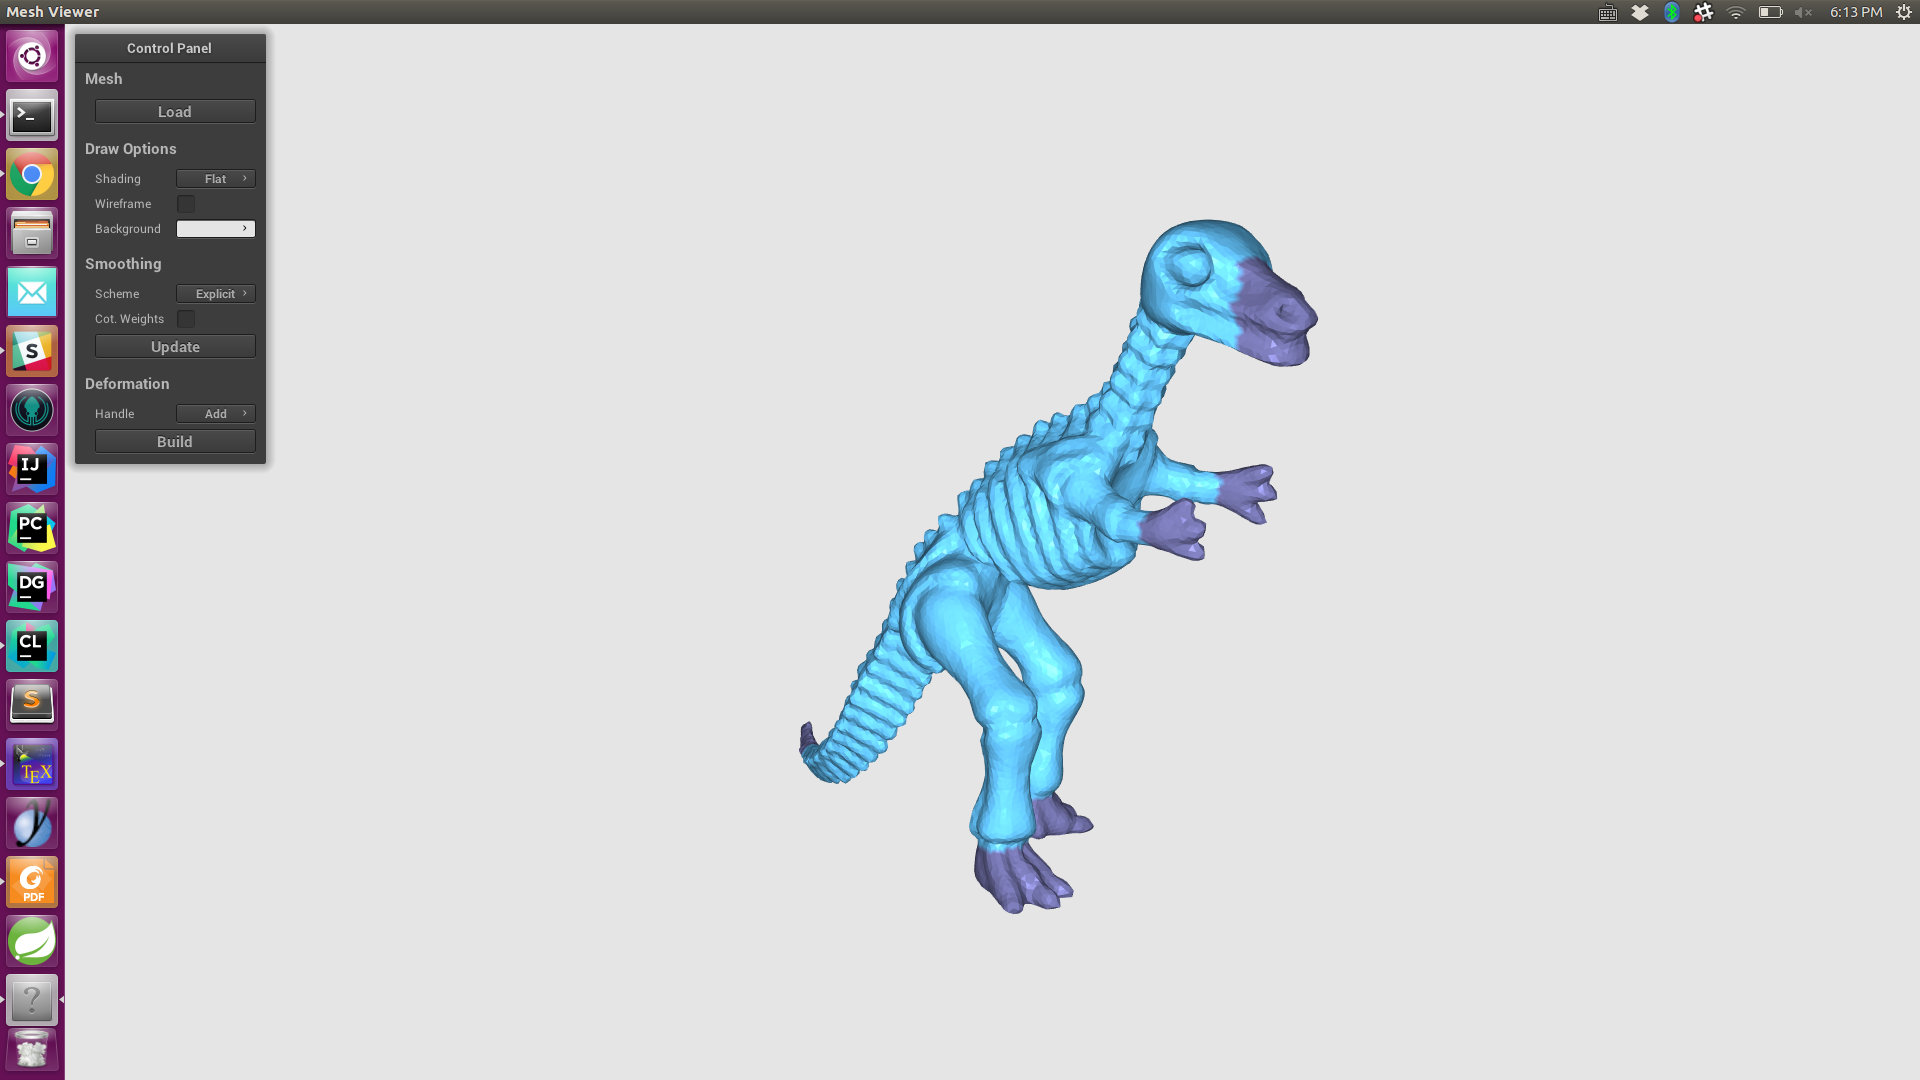
\includegraphics[width=1.0\linewidth]{dinosaur_before.png}
	\caption{original dinosaur}
\end{figure}
After editing:
\begin{figure}[H]
	\centering
	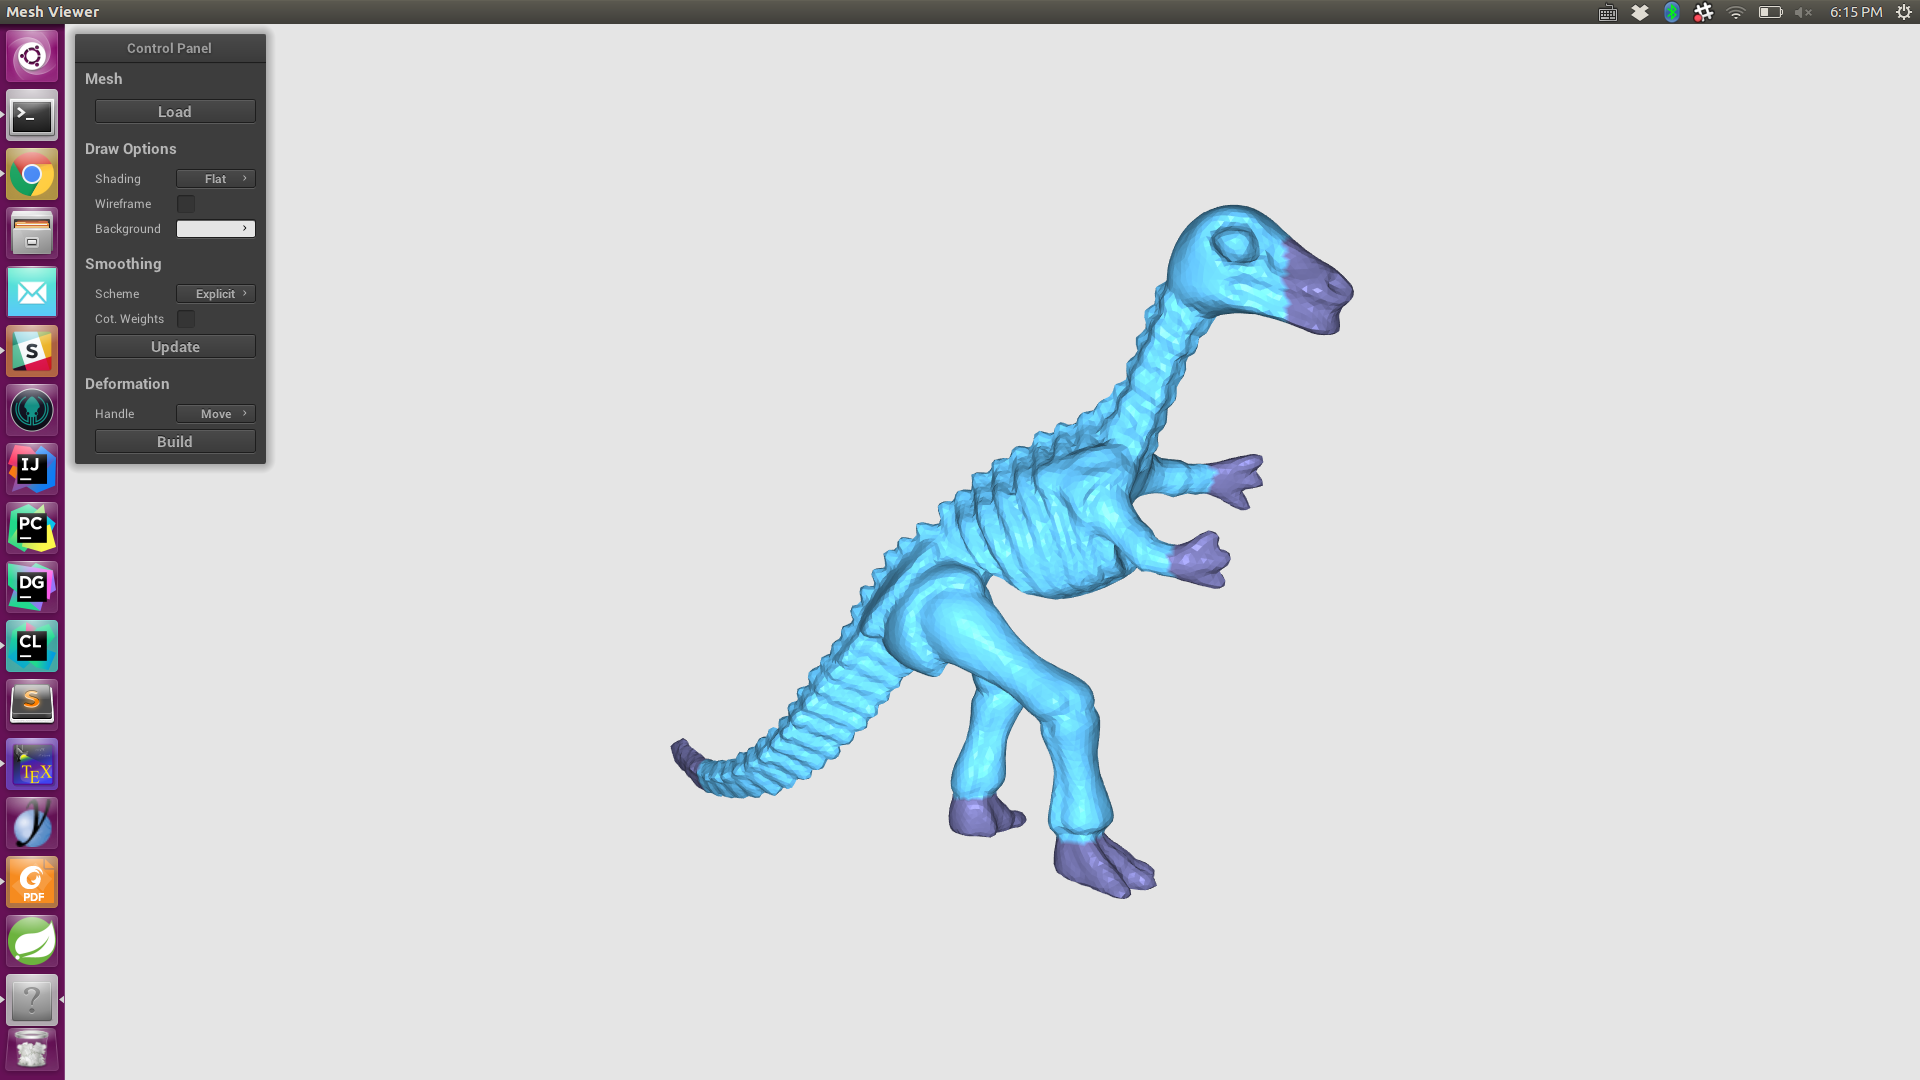
\includegraphics[width=1.0\linewidth]{dinosaur_after1.png}
	\caption{dinosaur after editing}
\end{figure}
\begin{figure}[H]
	\centering
	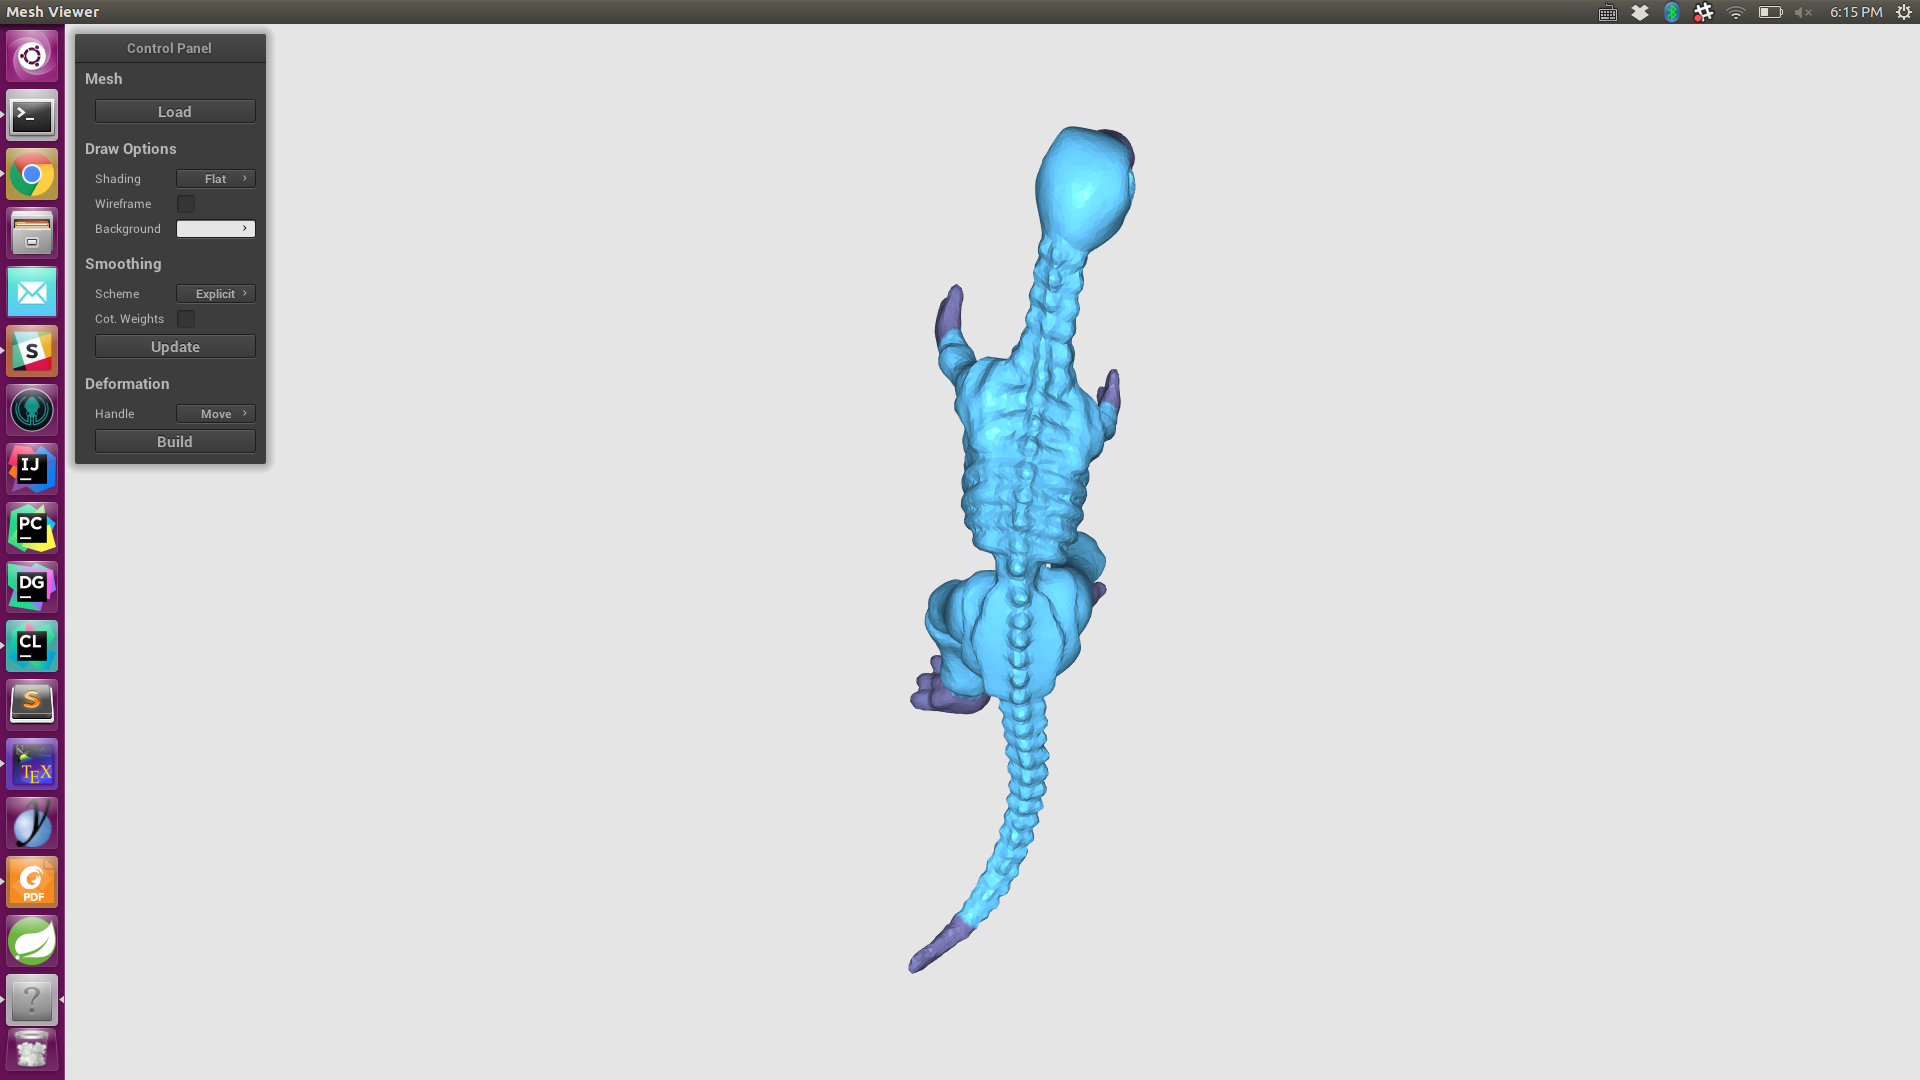
\includegraphics[width=1.0\linewidth]{dinosaur_after2.png}
	\caption{dinosaur after editing}
\end{figure}

\section{Laplacian Surface Editing on Feline}
Before editing:
\begin{figure}[H]
	\centering
	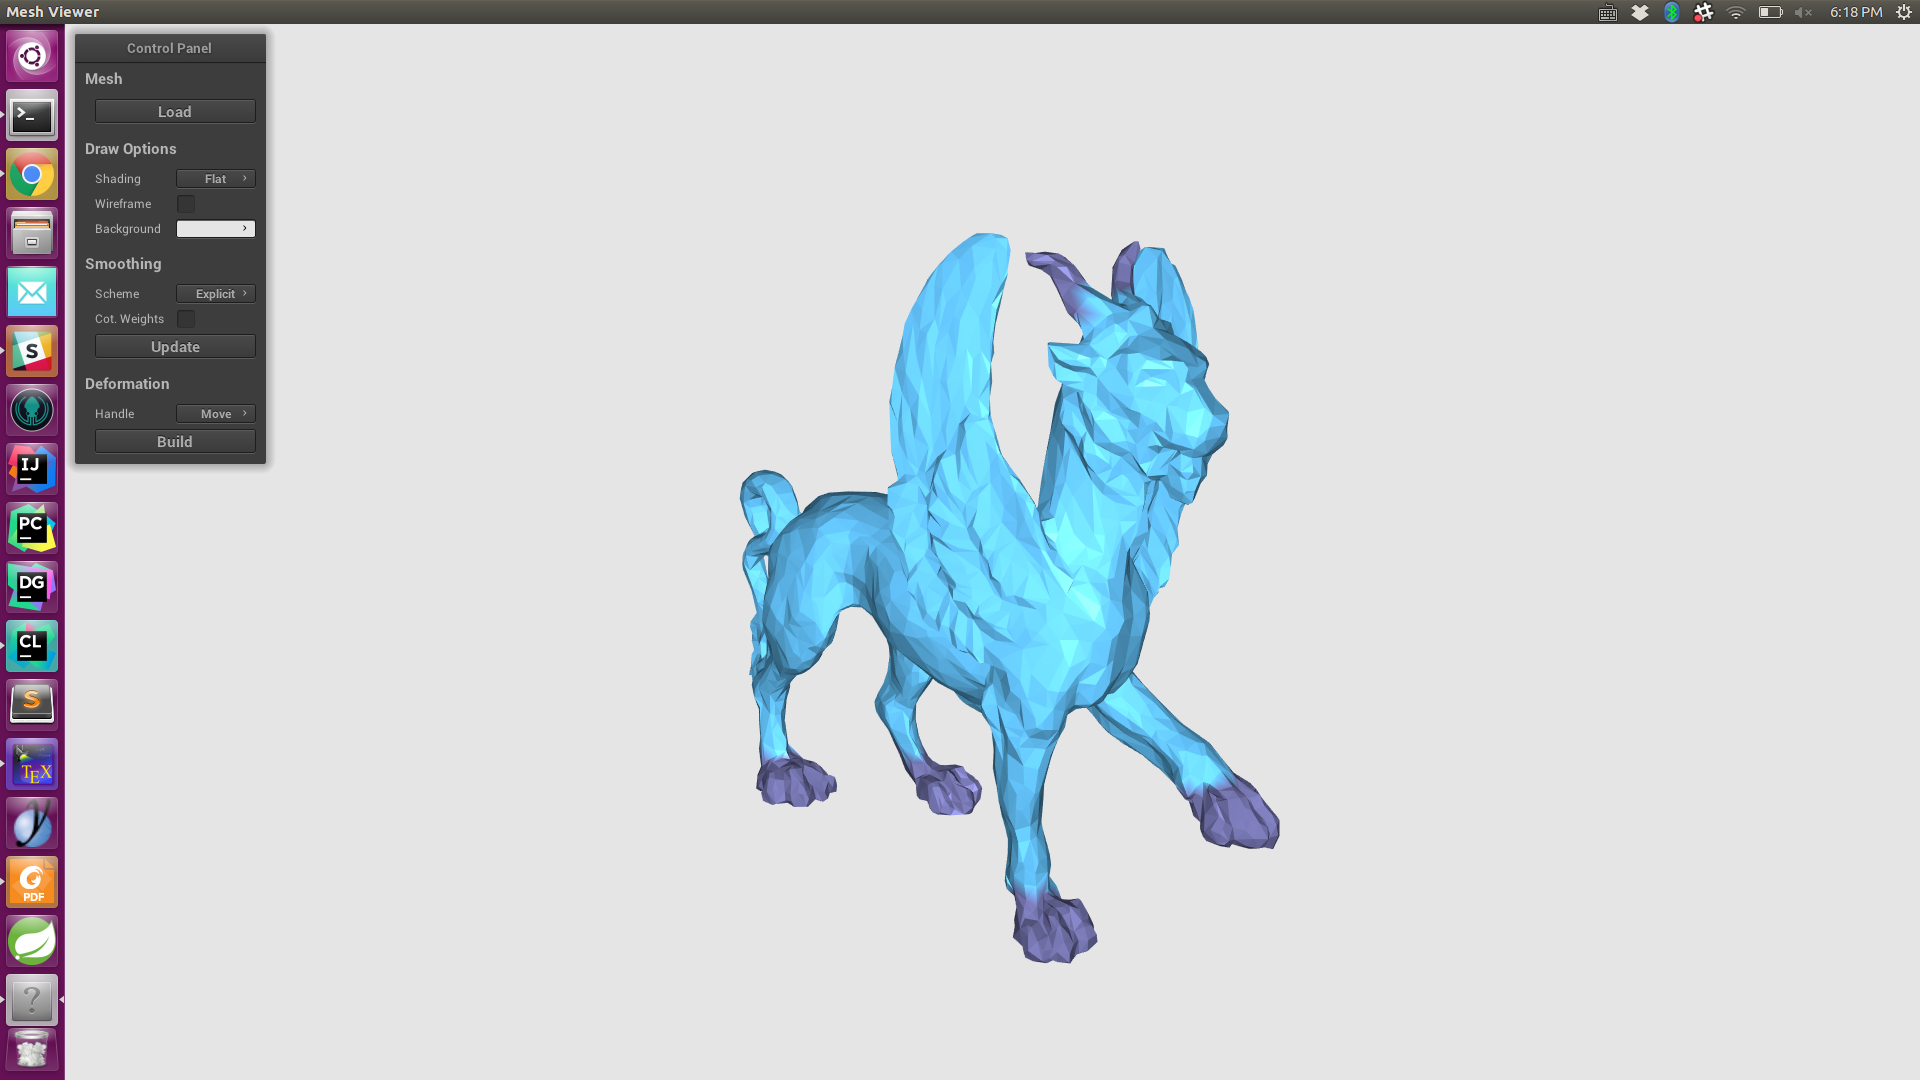
\includegraphics[width=1.0\linewidth]{feline_before.png}
	\caption{original feline}
\end{figure}
After editing:
\begin{figure}[H]
	\centering
	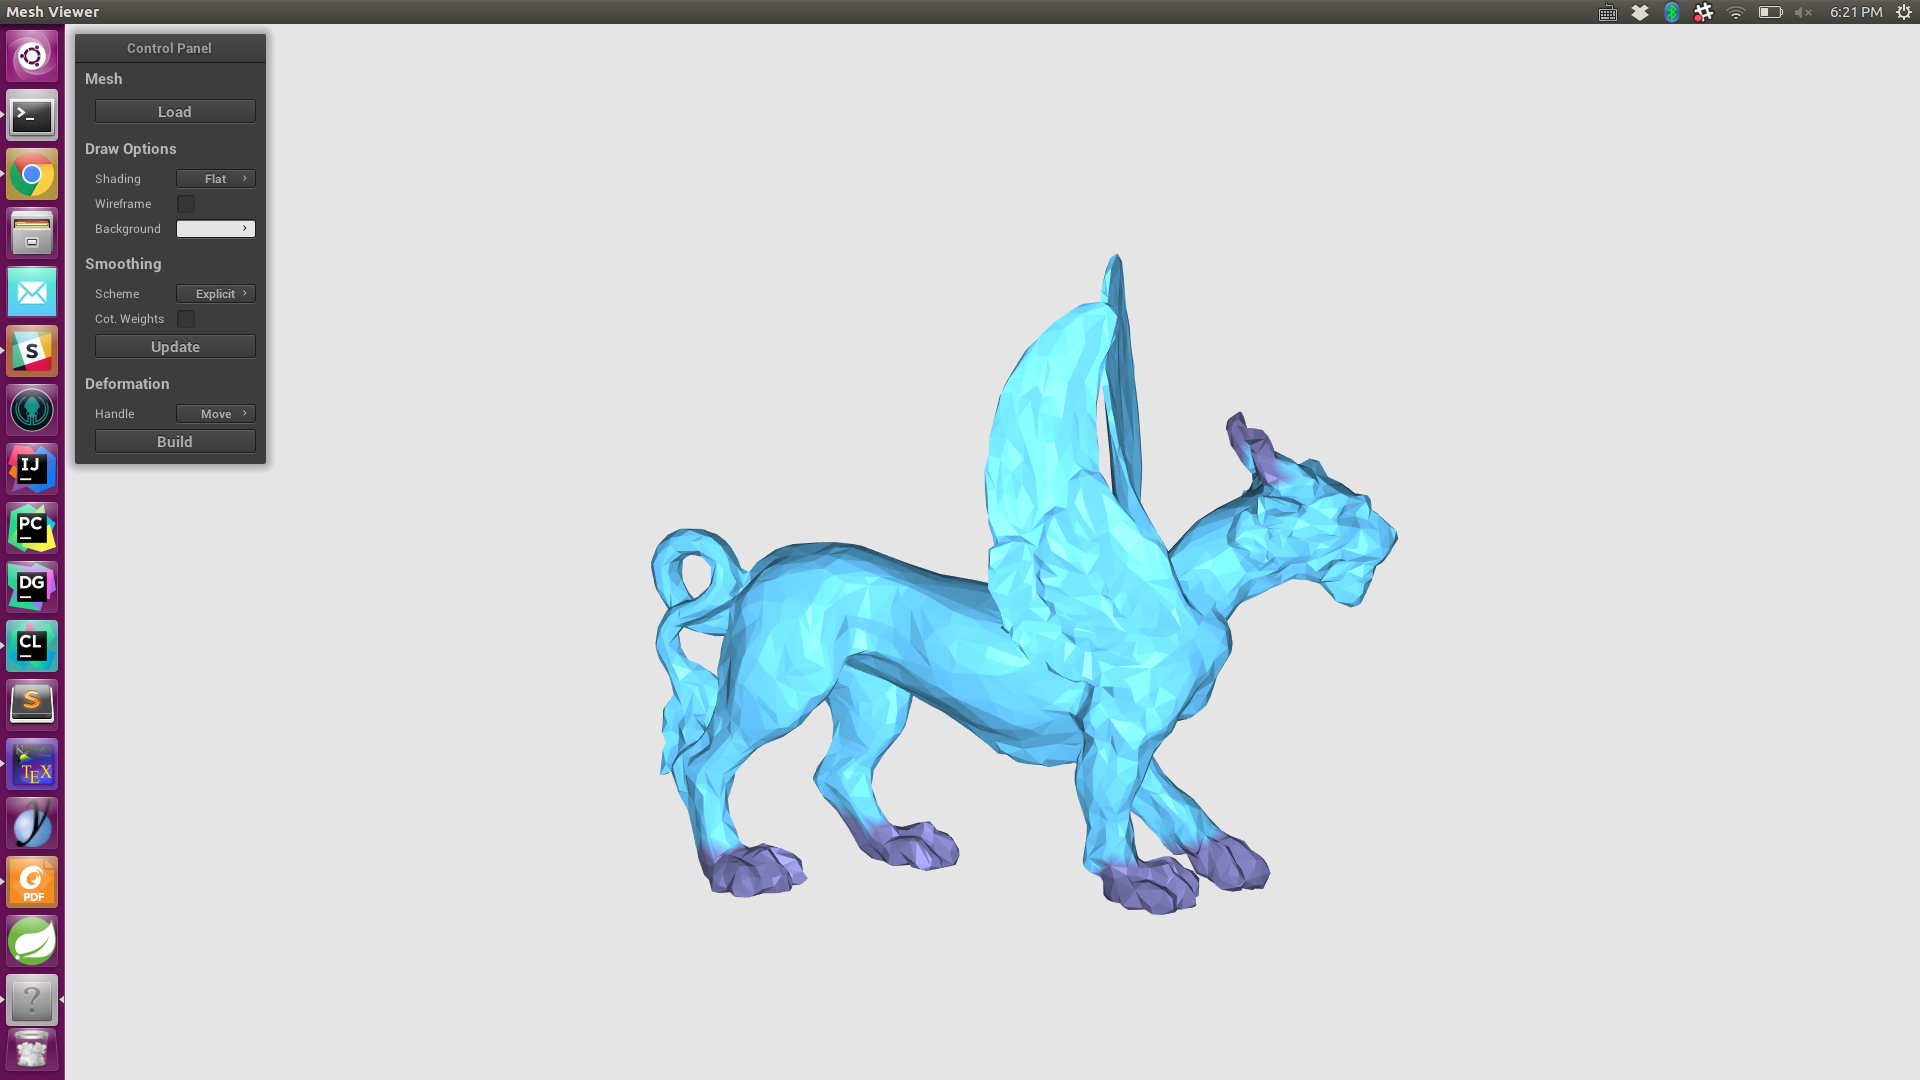
\includegraphics[width=1.0\linewidth]{feline_after1.png}
	\caption{feline after editing}
\end{figure}
\begin{figure}[H]
	\centering
	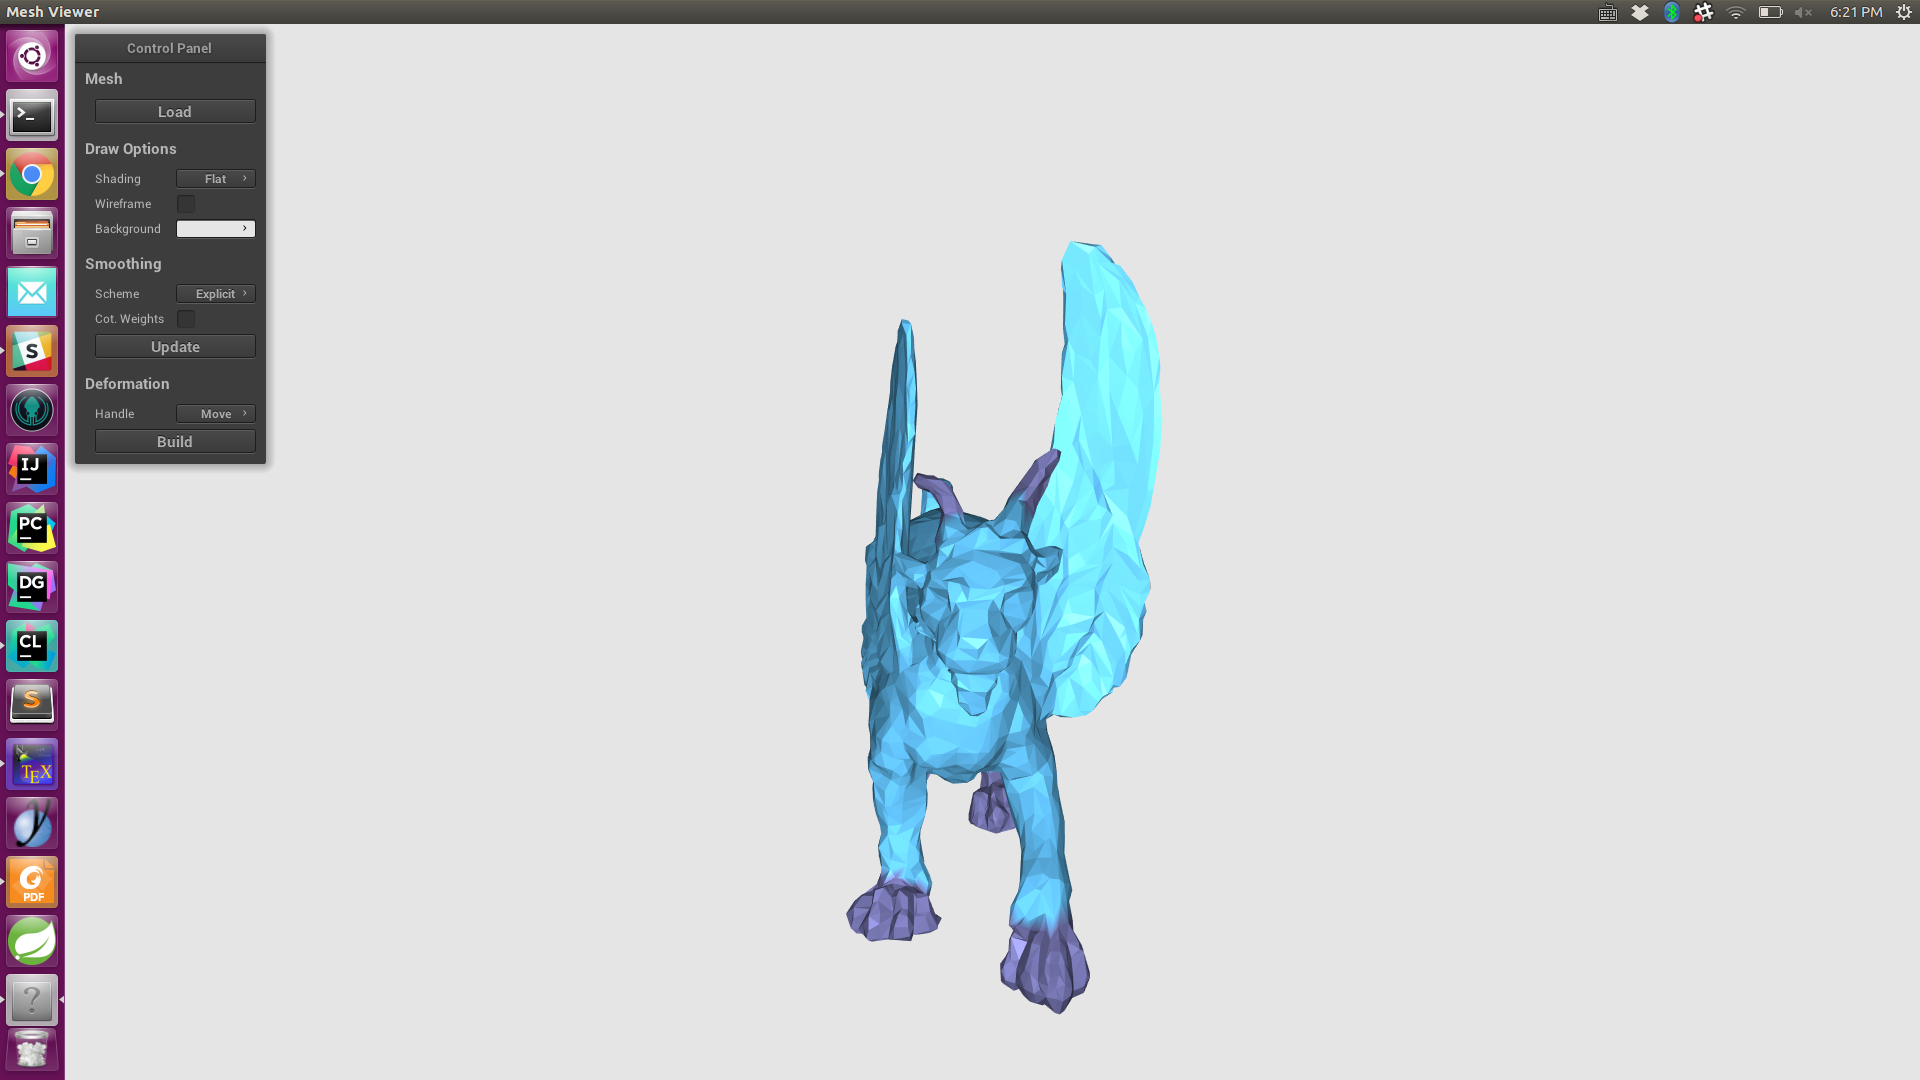
\includegraphics[width=1.0\linewidth]{feline_after2.png}
	\caption{feline after editing}
\end{figure}
\begin{figure}[H]
	\centering
	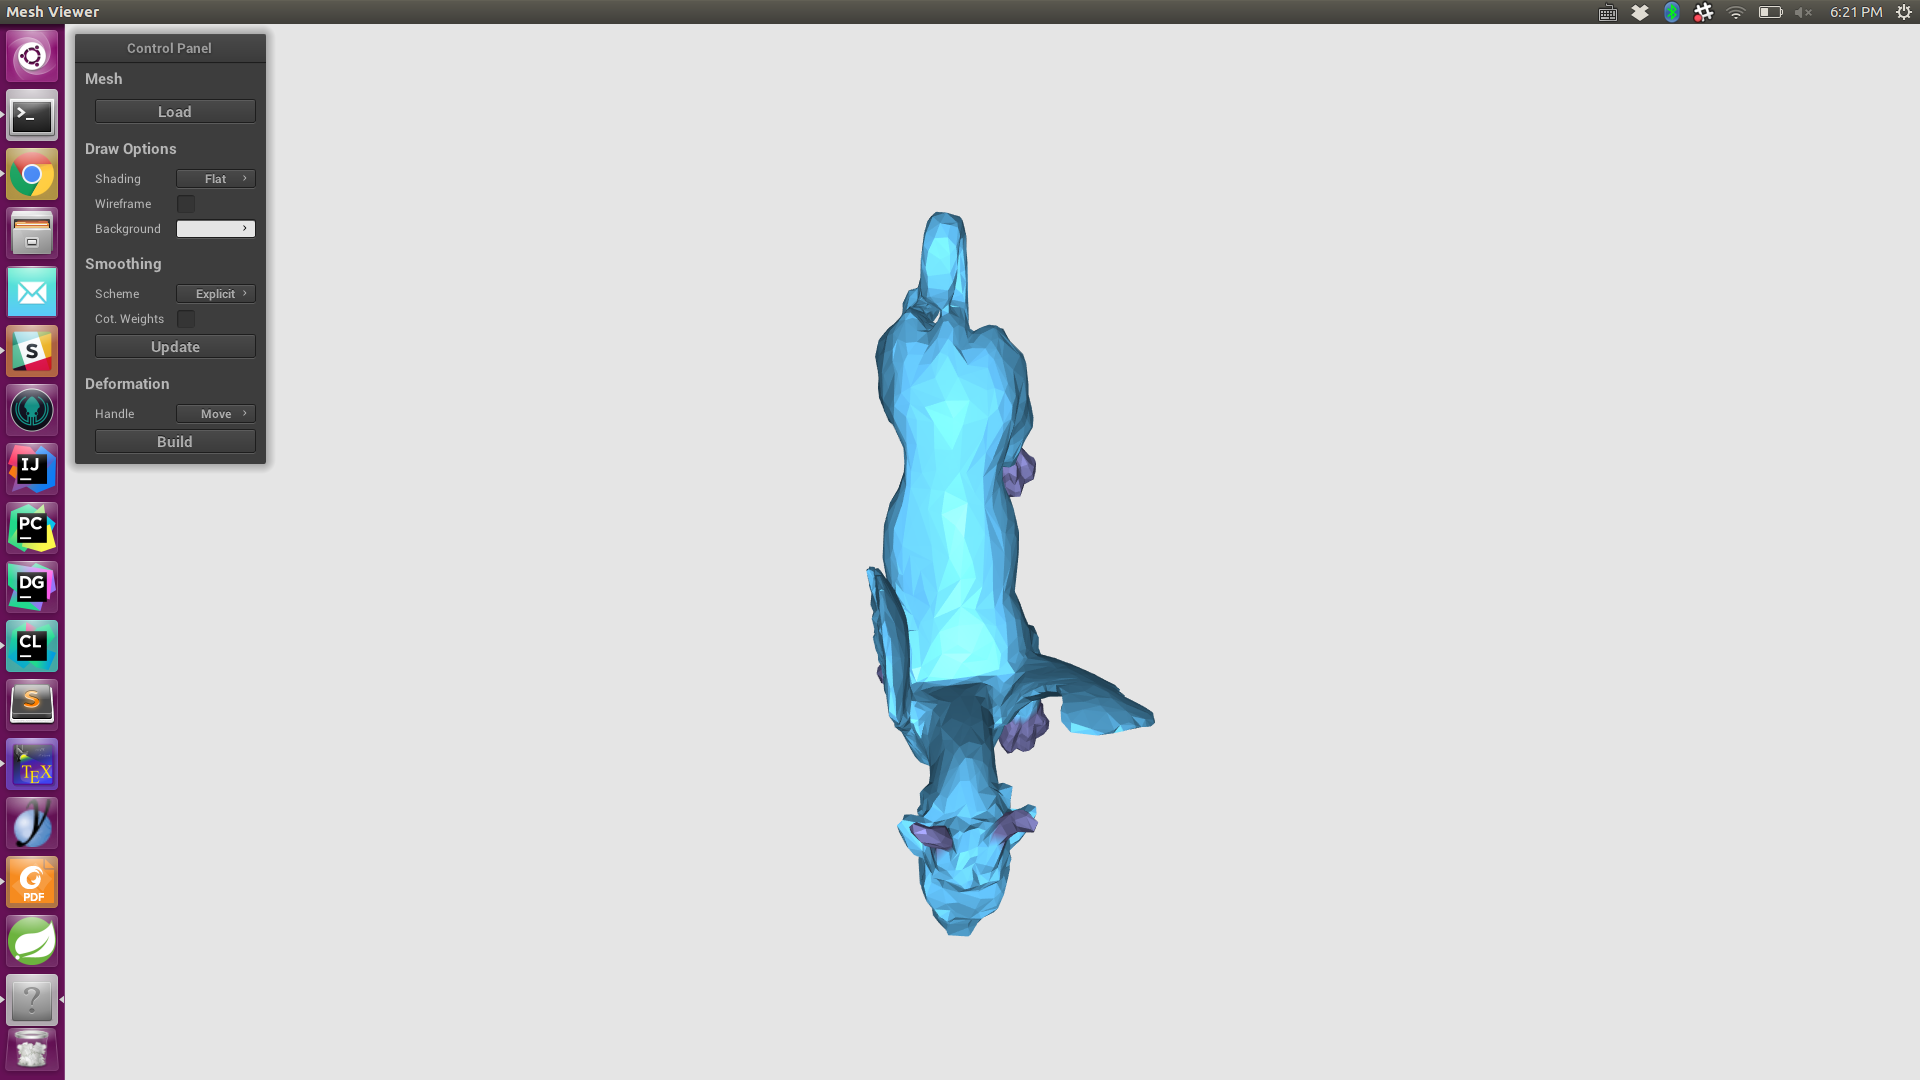
\includegraphics[width=1.0\linewidth]{feline_after3.png}
	\caption{feline after editing}
\end{figure}
\section{Laplacian Surface Editing on Knight}
Before editing:
\begin{figure}[H]
	\centering
	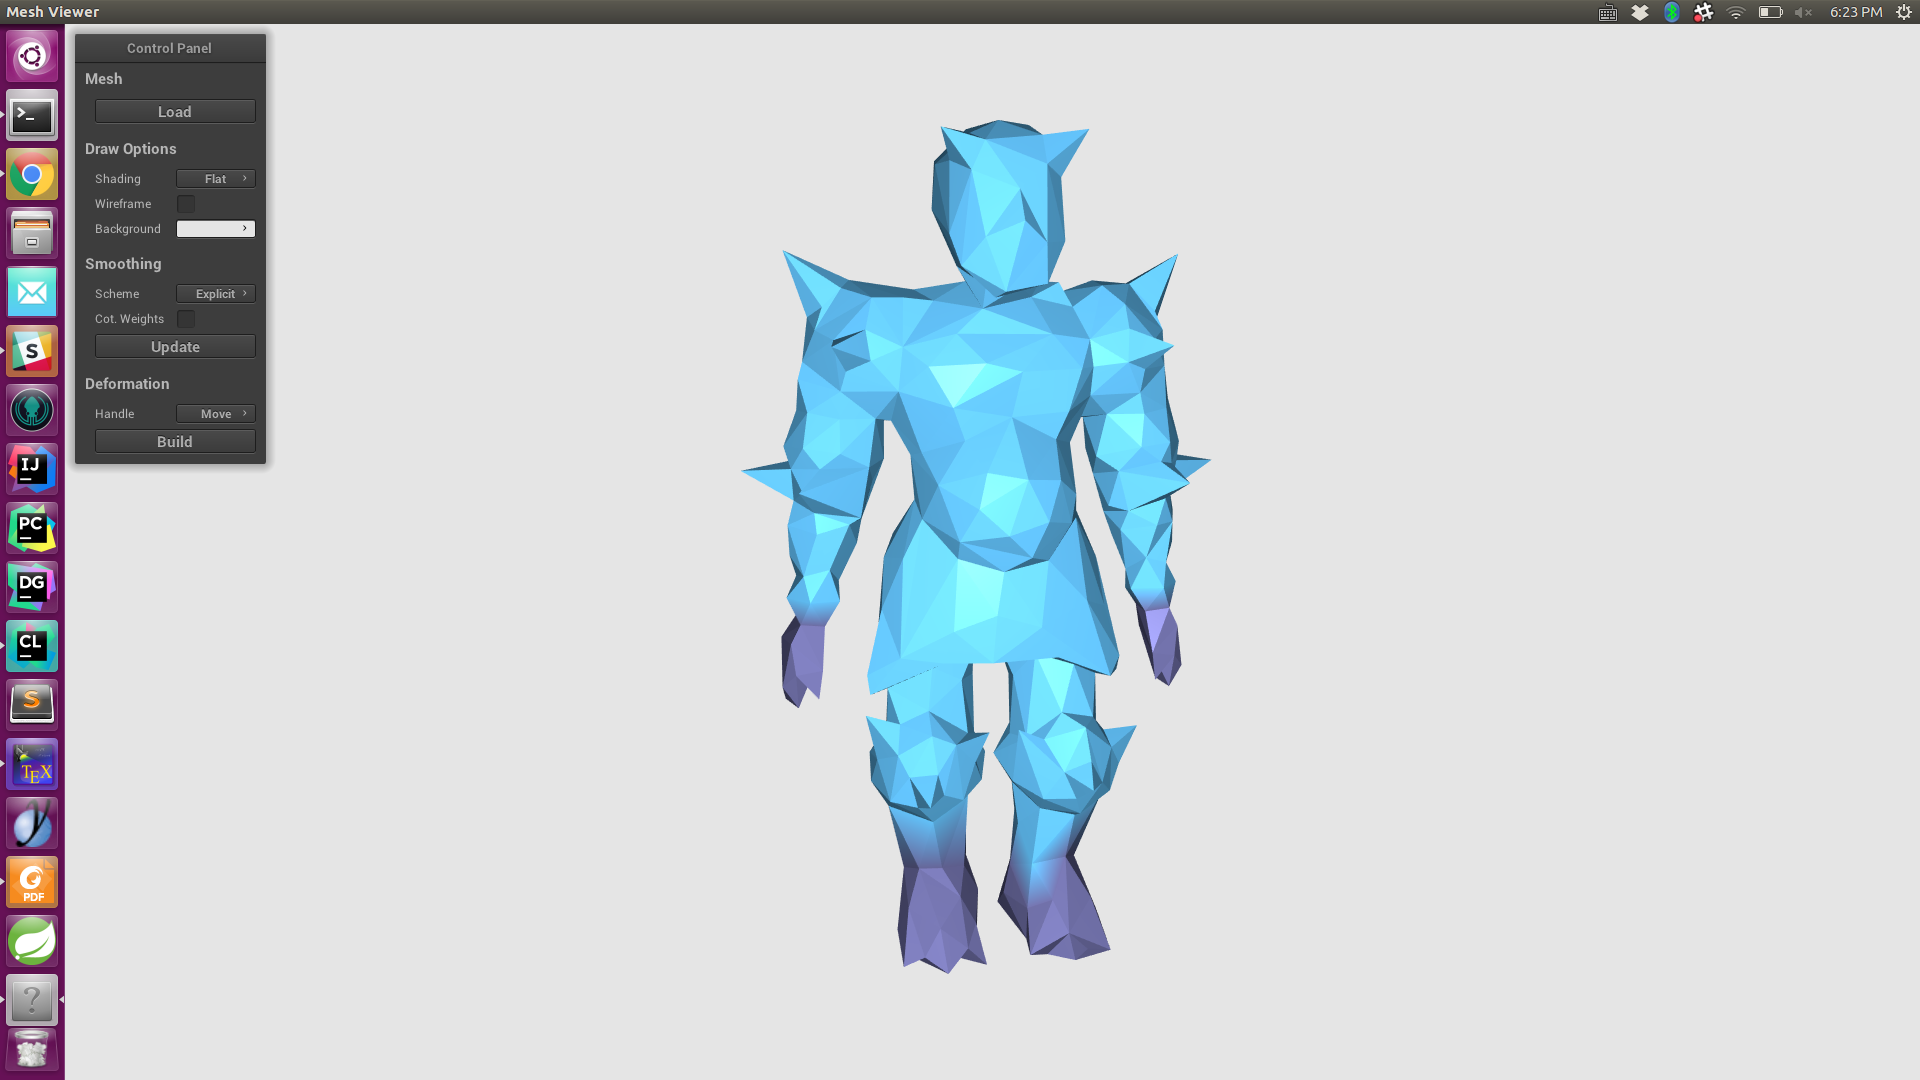
\includegraphics[width=1.0\linewidth]{knight_before.png}
	\caption{original knight}
\end{figure}
After editing:
\begin{figure}[H]
	\centering
	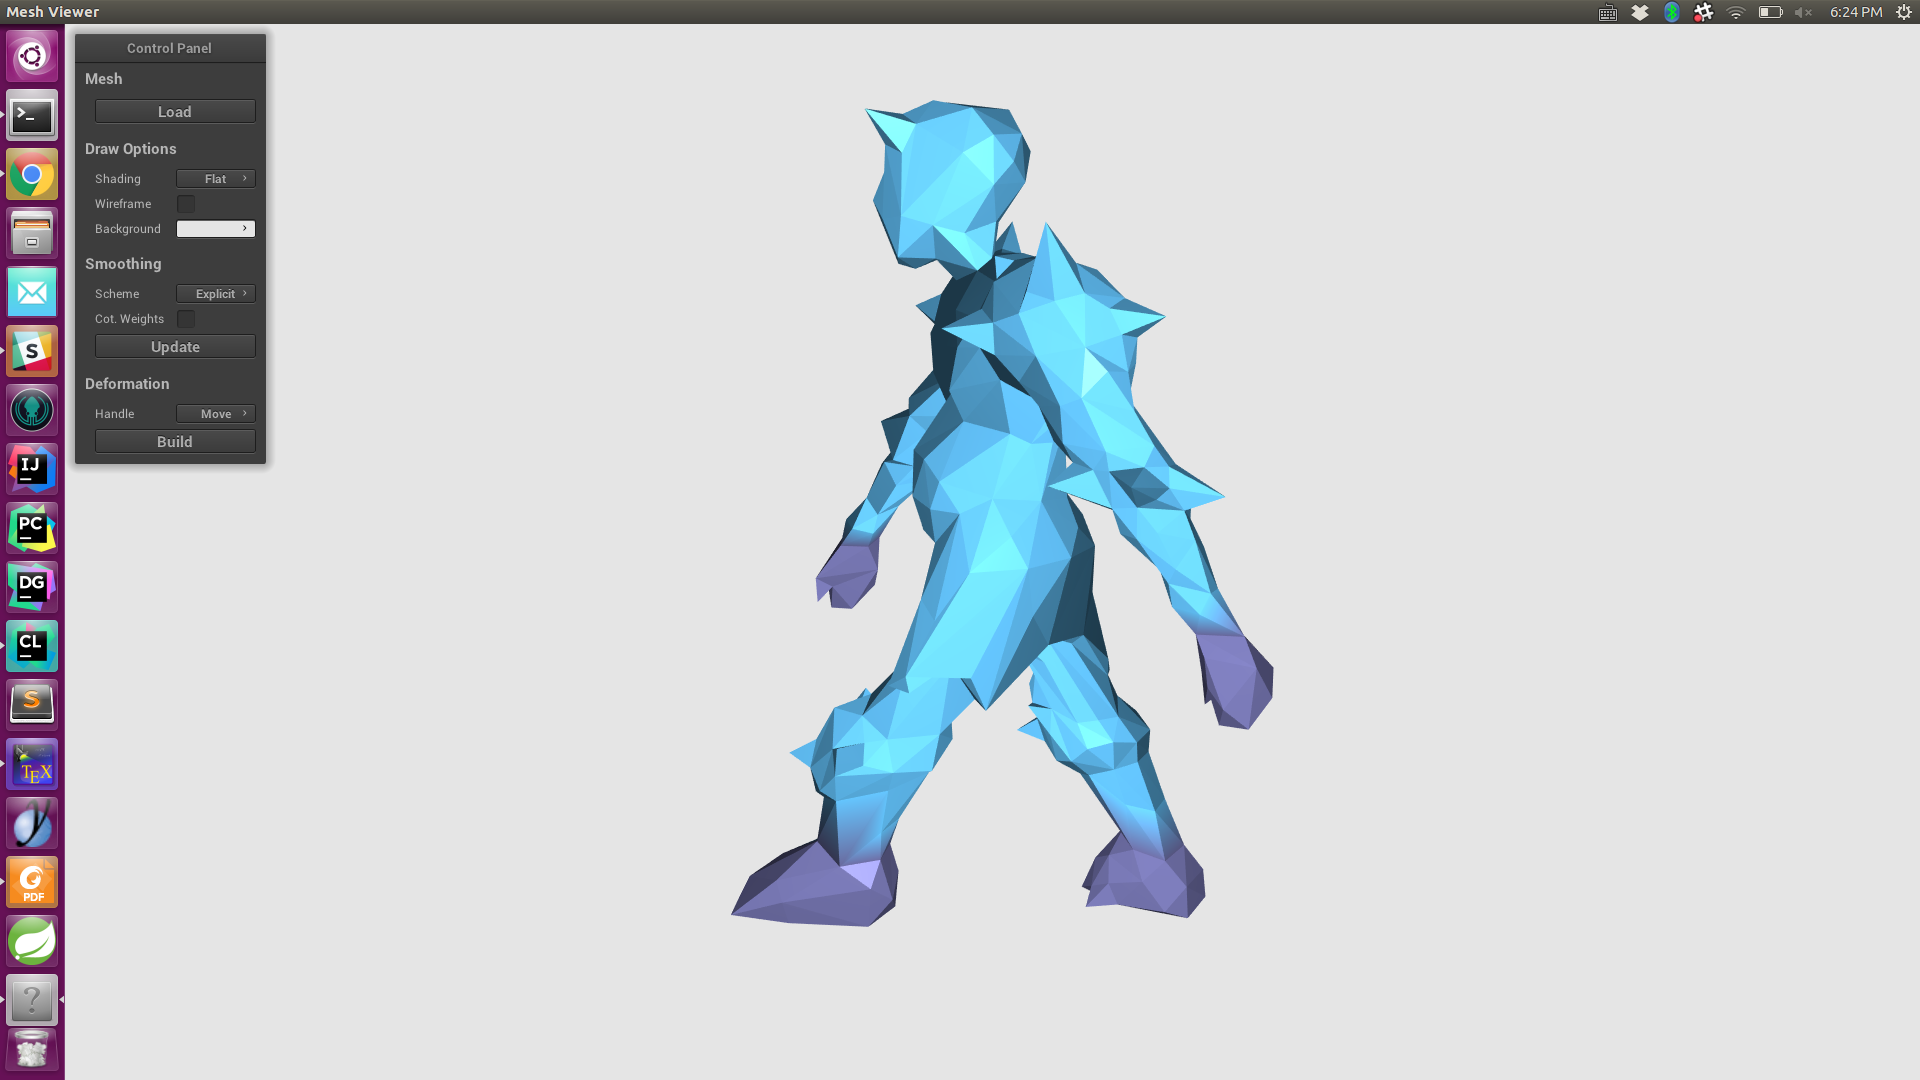
\includegraphics[width=1.0\linewidth]{knight_after1.png}
	\caption{knight after editing}
\end{figure}
\begin{figure}[H]
	\centering
	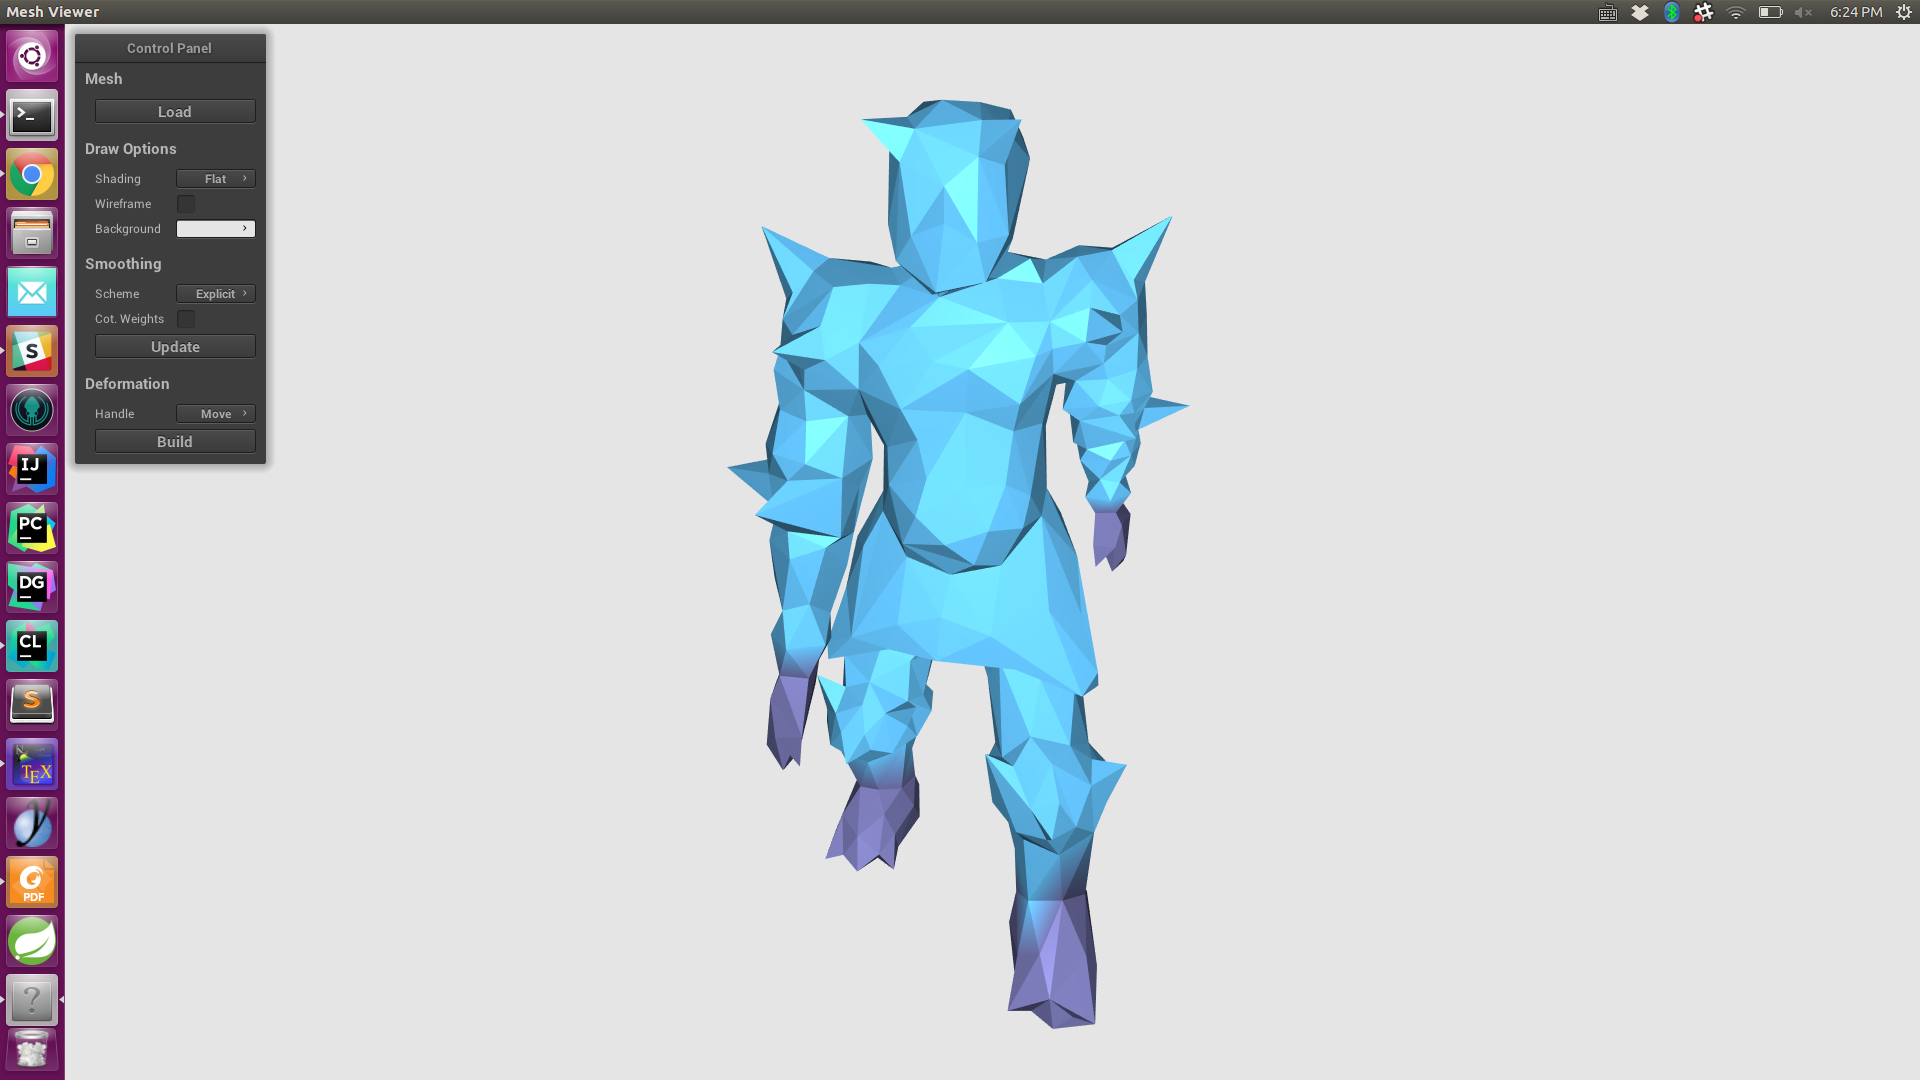
\includegraphics[width=1.0\linewidth]{knight_after2.png}
	\caption{knight after editing}
\end{figure}
\begin{figure}[H]
	\centering
	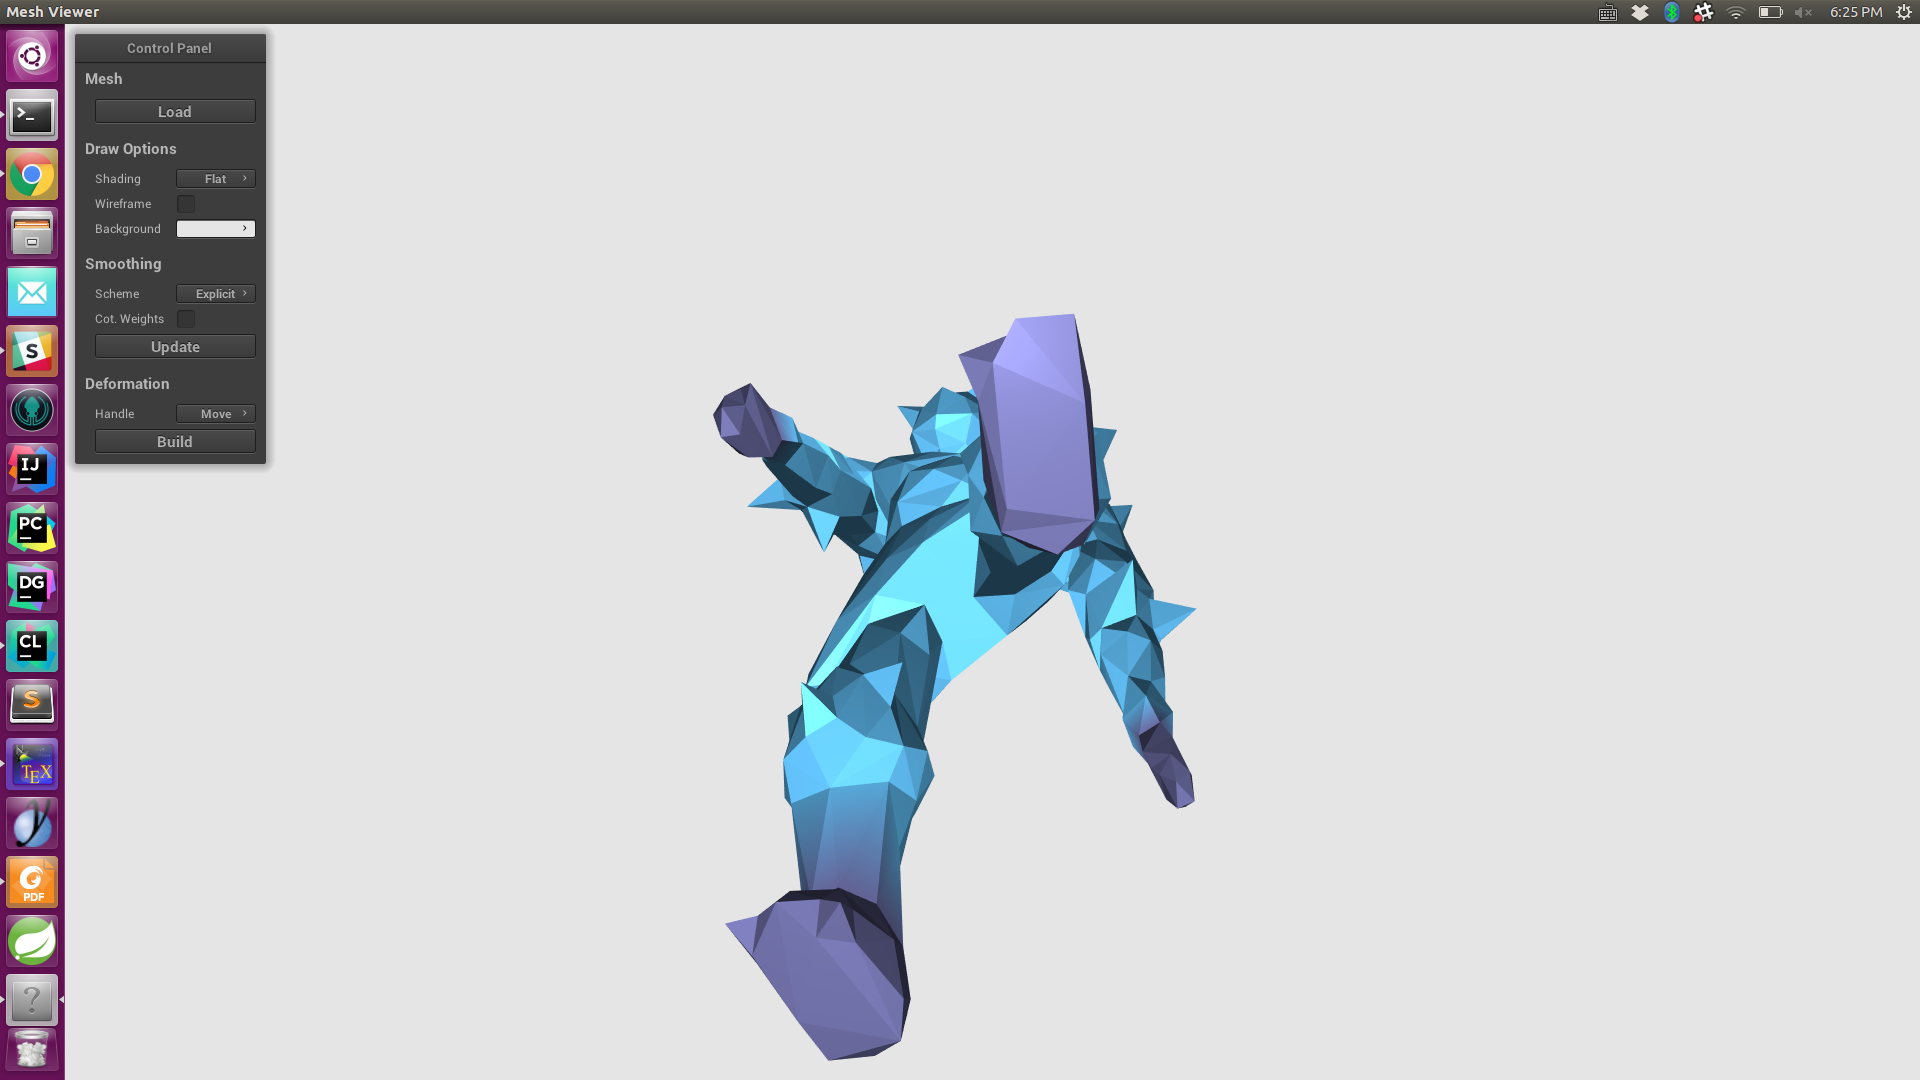
\includegraphics[width=1.0\linewidth]{knight_after3.png}
	\caption{knight after editing}
\end{figure}

\section{Conclusions}
From the result we can see that Laplacian surface editing preserves the object's surface shape when handles and boundaries are moved under constraints. However, from the result of knight after editing we can see that rotation is not automatically generated along the moving parts of the object if we are using the naive Laplacian surface editing.

\end{document}
